\documentclass[12pt,fleqn]{article}\usepackage{../common}
\begin{document}
Lineer Cebir - Ders 1

Ilk dersimize hosgeldiniz, ben Gilbert Strang. Lineer cebirin cozmeye
calistigi en temel problem bir lineer denklem sistemini cozmektir. Bu
baglamda mesela en genel durum ``bilinmeyen ve denklem sayisinin birbirine
esit oldugu'' durumdur, ki bu ``guzel durum'' olarak nitelenebilir. Boyut
$n \times n$ olunca bu durumda oluyoruz. Ama diger durumlari da
isleyecegiz. 

Dersin kavramlarini anlamak icin  ``satir bakisi''na basvuracagiz, bu
durumda her denkleme teker teker bakiyoruz gibi olacak, dersimizde pek cok
kez kullanacagimiz $A$ matrisimiz olacak mesela, ve bu matrisin satirlarin
her denklemin degiskenlerinin katsayilarina tekabul edecek.

Kolon bakis acisi belki daha once gormediginiz bir aci olacak, bu durumda
her kolon ayri ayri islenecek. 

Cebirsel bakis acisi ise tum matrisi, bu durumda $A$, ayni anda ele alacak.

Guzel durumdan baslayalim; iki bilinmeyen, iki denklem.

$$ 2x - y = 0 $$

$$ -x + 2y = 3 $$

Katsayilari matrise tasiyalim

$$ 
\left[\begin{array}{cc}
2 & -1 \\
-1 & 2
\end{array}\right]
\left[\begin{array}{c}
x \\
y
\end{array}\right]
=
\left[\begin{array}{c}
0 \\
3
\end{array}\right]
 $$

Soldaki matrise ben cogunlukla $A$ derim, sonra icinde bilinmeyenleri
tasiyan $x$ vektoru koyarim, ki bazilari bunu vektor oldugu icin koyu
renkte $\mathbf{x}$ olarak ta yazar, ve sonra bir vektor daha, ki buna ben
cogunlukla $b$ derim, yani sonuc soyle olur,

$$ A x = b $$

Simdi satir bakisina basvuralim. Grafik olarak dusunelim, hangi noktalar
$2x - y = 0$ denklemini tatmin eder? Orijin $(0,0)$ noktasi bunlardan biri,
bir digeri $x=1,y=2$. Bunlari cizgi ile birlestirip cizgiyi sonsuza uzatirsak,

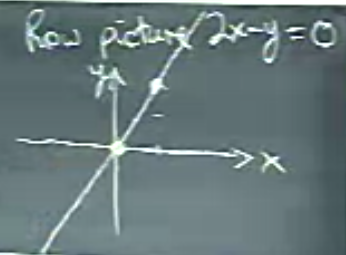
\includegraphics[height=4cm]{1_01.png}

Ikinci denklemi dusunelim, bu denklem orijinden gecmeyecek. $y$ sifir
olsaydi $x$ nereden gecerdi..? $x=-3$ noktasindan. $x=-1$ ise, $y$ nedir?
$y=1$. Artik ikinci cizgiyi cizebiliriz,

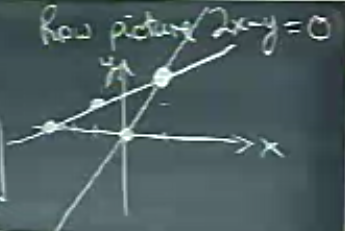
\includegraphics[height=4cm]{1_02.png}

Her iki cizgi $x=1,y=2$ noktasinda bulustu (hoca o noktayi daha onceden
tahtaya koymustu ama buna bir ``hazir raslanti'' diyelim). Bu bulusma
noktasi her iki denklemi tatmin eden sistemin cozum noktasidir.

Kolon bakisina gelelim. Bu bakisa gore

$$ 
x
\left[\begin{array}{r}
2 \\
-1
\end{array}\right]
+
y
\left[\begin{array}{r}
-1 \\
2
\end{array}\right]
=
\left[\begin{array}{r}
0 \\
3
\end{array}\right]
$$

Bu bakis acisi bize ne soyluyor? Bir anlamda diyor ki ``esitligin solundaki
iki vektoru oyle bir sekilde kombine et ki bu lineer kombinasyon sonucu
esitligin sag tarafini versin''. Bu operasyon, islem lineer cebir dersinin
en temel islemidir - kolonlarin lineer kombinasyonu. 

Kolonlari vektorel olarak cizelim, bilindigi gibi bir vektor orijinden
cikan bir yonu ve buyuklugu olan bir seydir. Birinci kolon 2 saga 1 asagi
gitmeli, ikincisi bir sola 2 yukari gitmeli. Cizince,

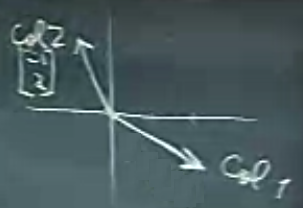
\includegraphics[height=4cm]{1_03.png}

Peki bu vektorleri nasil ``birlestirelim'' yani hangi katsayilarla carpip
toplayalim ki $\left[\begin{array}{rr}3 & 0\end{array}\right]^T$ sonucunu
elde edelim? Not: Burada devrik isaretini kullandik cunku satir vektorunun
devrigini alinca kolon vektoru olur, yazarken o sekilde yazdik cunku baska
turlu yazi icine rahat koymak mumkun olmayacakti.

Neyse, kombine etmek toplamaktir, o zaman ikinci kolonu alip birinciye
ekleyelim, vektor aritmegitinde toplamak bir vektoru digerinin bittigi
noktadan baslatmak demektir, bir tane (yani katsayi 1 ile) ikinci vektoru
birinciye ekleyince

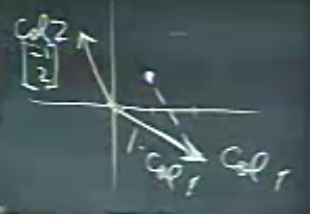
\includegraphics[height=4cm]{1_04.png}

Cozum noktasina erisemedik daha, 2 tane ekleyince,

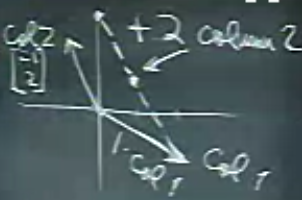
\includegraphics[height=4cm]{1_05.png}

Cozume eristik. Cozum $y$ ekseni uzerinde 3,0 noktasi. Bu noktaya bir
lineer kombinasyon yaparak eristik. ``Dogru'' lineer kombinasyon bize
sonucu verdi. 

Kendimize sunu soralim: {\em butun} lineer kombinasyonlar bize neyi
verirdi? Bu cok onemli bir soru, uzerinde iyi dusunelim, cunku bu konu
tekrar tekrar karsimiza cikacak. Tum kombinasyonlar derken tum $x,y$'lerin
doguracagi kombinasyonlar; bu sekilde esitligin sag tarafi ne olursa olsun
onu temsil edebilirdik. Yani bu tum kombinasyonlar tum bir duzlemi (plane)
doldururdu. Bunu bir kenara koyalim, konuyu ileride daha detayli olarak
inceleyecegiz.

3 Boyut

$$  2x - y = 0  $$

$$ -2x + y - z = -1 $$

$$ -3y + 4z = 4 $$

Bu sistemi nasil anlariz? Ne gorduk: satir bakisi, kolon bakisi. Matris
formuna bakalim, 

$$ A = 
\left[\begin{array}{rrr}
2 & -1 & 0 \\
-1 & 2 & -1 \\
0 & -3 & 4 
\end{array}\right]
,
b = 
\left[\begin{array}{r}
0  \\
-1 \\
4  
\end{array}\right]
 $$

Satir bakisi, ustteki ikinci denklemi alalim, grafigi neye benzer?
Orijinden gecen bir sey yok, cunku $0,0,0$ bir cozum olamaz. Cozum neye
benzer? Elimizde bir lineer denklem var ise uc boyutta bu denklemi cozen
tum noktalar bir duzlem (plane) olustururlar. Hoca diyor ki ben Rembrandt
degilim, kabaca bir duzlem cizecegim, 

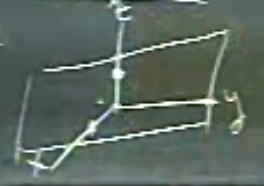
\includegraphics[height=4cm]{1_06.png}

Birinci denklem neye benzer? $z$ belirtilmemis, demek ki herhangi bir sey
olabilir, geri kalanlar yine bir duzlem olustururlar. Mesela alttaki gibi

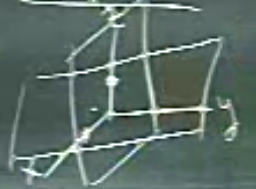
\includegraphics[height=4cm]{1_07.png}

Bu iki denklemin kesistigi yer bir cizgidir (line). Bir ucuncu duzlem daha
eklenince (ustte yok), tum uc duzlemin kesistigi yer bir nokta olur. Bu
noktanin ne oldugunu ben kafadan bilmiyorum, ama lineer cebir bu noktayi
bulur.

Fakat herhalde goruyorsunuz, satir bakisini zihnimizde canlandirmak biraz
zor. Duzlemler, kesismeler vs dusunmemiz gerekiyor. Iki boyutta iki cizgi
kesismesinde problem yoktu, fakat uc boyutta isler biraz karisti. Dort ya
da daha fazla boyutu dusunun! 

Kolon bakisi ile

$$ 
x 
\left[\begin{array}{r}
2 \\
-1 \\
0
\end{array}\right]
+
y
\left[\begin{array}{r}
-1 \\
2 \\
-3
\end{array}\right]
+
z 
\left[\begin{array}{r}
0 \\
-1 \\
4
\end{array}\right]
=
\left[\begin{array}{r}
0 \\
-1 \\
4
\end{array}\right]
 $$

Yani esitligin sol tarafindaki uc boyutlu vektorlerin hangi kombinasyonu
esitligin sagindaki uc boyutlu vektoru verir? Cizmeye ugrasalim,

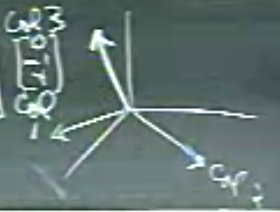
\includegraphics[height=4cm]{1_08.png}

Hocanin hazirladigi ornekte basit bir cozum var, $z$ katsayilari ile $b$
ayni, o zaman $[0,0,1]$ denklemi cozer, $z=1$ cozum icin yeterli olur,
$z$'yi aliriz, geri kalanlari ``istemiyoruz'' onlari sifir yapariz -
$x=0,y=0,z=1$.

Tabii kolon resminin daha duzgun olmasi her zaman cozumu pat diye
gorebilecegimiz anlamina gelmiyor, cogu zaman, hatta yuksek boyutlarda bu
da mumkun degil. Eliminasyon yontemini gorecegiz ileriki derslerde,
sistematik olarak herhangi bir boyutta bizim icin lineer sistemi cozecek. 

Daha genis resme bir bakalim. Esitligin sag tarafi baska bir sey olsaydi,
mesela

$$ 
x 
\left[\begin{array}{r}
2 \\
-1 \\
0
\end{array}\right]
+
y
\left[\begin{array}{r}
-1 \\
2 \\
-3
\end{array}\right]
+
z 
\left[\begin{array}{r}
0 \\
-1 \\
4
\end{array}\right]
=
\left[\begin{array}{r}
1 \\
1 \\
3
\end{array}\right]
 $$

(Bu sag tarafi 1. ve 2. kolonlari birbirine ekleyerek uydurduk bu arada),
cozum o zaman ne olurdu? Cozum basit (cunku kendimiz pisirdik),
$x=1,y=1,z=0$. Ustteki durumda ve satir bakisinda tamamen degisik uc tane
duzlem elde ederdik. Kolon bakisinda hala ayni uc vektorle ugrasiriz,
sadece onlari degisik sekillerde kombine etmemiz gerekir. 

Soru: ustteki denklemi herhangi bir $b$ yani esitligin sag tarafi icin
cozebilir miyim? 

Bu soruyu daha degisik bir sekle sokabilir miyiz, oyle ki soru lineer
kombinasyon argumanlarini kullansin. 

Soru: ustteki kolonlarin lineer kombinasyonu butun 3-boyutlu uzayi doldurur
mu?

Cevap, ustteki (gibi bir) matris icin ``evet''. Bu matris nasil bir matris?
Bu matris iyi huylu, tekil (singular) olmayan, tersi alinabilir
(invertible) bir matris. Bu tur matrisler icin her zaman cozum var. 

Peki iyi huylu olmayan durum nasil olurdu? Dusunelim, ne yanlis
gidebilirdi? Eger tum vektorler ayni duzlem uzerinde olsaydilar, o zaman bu
vektorlerin her turlu kombinasyonu da ayni duzlem uzerinde olmak
zorundadir, o zaman basimiz dertte. Mesela 3. kolon 1. ve 2.'nin toplami
olsa (ki bu durumda her uc vektor ayni duzlemdedir), o zaman isler
kotu. Niye? Cunku $b$ farkli bir duzlemde ise artik hicbir kombinasyonla
oraya erisemem. Eger $b$ ayni duzlem uzerinde olsaydi tabii erisilebilirdi,
yani {\em bazi} $b$'ler icin cozum hala var, ama hepsi, cogunlugu icin yok. 

Iste tekil durum budur, ki bu durumda cogu $b$ icin cozum yoktur.

Boyutlari arttirdigimizi dusunelim. 9 boyut olsaydi ne olurdu? Bu kadar
boyutu gorsel olarak hayal etmek mumkun degil, ama yine ayni durum, $Ax=b$
var, bu sefer 9 boyutlu 9 tane kolon var, bunlari kombine edip $b$ elde
edecegiz? Bunu yapmayi basarabilmemiz tabii ki $A$'nin ne olduguna
baglidir. Rasgele bir $A$ matrisi uretseydim (ki bu Numpy \verb!rand! ile
basitce yapilabilir) size garanti ediyorum bu matris iyi huylu olurdu,
tekil olmayan tersi alinabilen vs. ve bu matris ile $b$'ye
erisebilirdiniz. 

Kotu durum kolonlar bagimsiz olmadigi zaman. Mesela 7. kolon 5. kolonun
tipatip aynisi, ki bu durumda 7. kolon sisteme ``yeni hic bir bilgi
eklemiyor''. Bu yuzden bazi $b$'lere erismem imkansiz hale geliyor. Iyi
huylu durumda 9 bagimsiz kolonun kombinasyonu tum 9 boyutlu uzayi
doldurabilirdi. Ama bir bagimli vektor var ise o zaman sadece 9 boyutlu
uzayin 8 boyutlu bir alt duzlemini doldurabilirsiniz. Dersimizin ileri
noktalarinda bu kisitli alt uzaylar ile de is yapmayi ogrenecegiz, yapmamiz
gerekecek. Simdilik guzel kosula odaklanalim.  

Ayrica, simdiye kadar sozel olarak belirttiklerimizi bir de matris
formunda, cebiriyle anlatmayi deneyelim. $Ax=b$ dedik, $A$ matrisi bir $x$
vektoru ile carpilir. Bir vektoru bir matris ile nasil carparsiniz? Mesela

$$ 
\left[\begin{array}{rr}
2 & 5 \\
1 & 3
\end{array}\right]
\left[\begin{array}{r}
1 \\
2
\end{array}\right]
 $$

Bunu yapmanin iki yolu var. Once benim en favori yontemimi soyleyeyim,
belki de surpriz olmayacak, kolonlar kullanarak. Bu durumda, mesela ustteki
ornekte, $A$'nin 1. kolunundan 1 tane, 2. kolonundan 2 tane alacagim, ve
toplayacagim. Yani,

$$ =
1
\left[\begin{array}{r}
2 \\
1
\end{array}\right]
+
2
\left[\begin{array}{r}
5 \\
3
\end{array}\right]
=
\left[\begin{array}{r}
12 \\
7
\end{array}\right]
 $$

Diger bir yontem satir bazli. Bu durumda $A$'nin 1. satiri ile $x$'i
carpiyorum, yani noktasal carpimini aliyorum, ve bu tek bir deger sonucunu
verecek, ve tek, skalar degeri alip sonucun ilk hanesine yaziyorum. Ayni
sekilde $A$'nin 2. satirini tekrar ayni $x$ ile noktsal carpiyorum, ikinci
haneye yaziyorum. 

Fakat daha once belirttigimiz gibi kolon bakisi biraz daha rahat
aciklanabilir halde. O zaman sunu soyleyebiliriz: ``$Ax$, $A$'nin
kolonlarinin bir kombinasyonudur''. 

Bir sonraki derste herhangi boyuttaki bir sistem icin sistematik olarak
eliminasyon yaparak, eger varsa, bir sonuca ulasmayi ogrenecegiz. Eger
eliminasyon basarisiz olursa bunun uzerinden ne zaman bir sonuc olmadigini
gormeyi de ogrenecegiz. 



\end{document}
